\section{Background Theory}
% Describe the essential theory or theories to be applied in the thesis.

\subsection{Formal methods}
Formal methods are techniques used to model complex systems as
mathematical entities.

The primary idea behind a formal method is that there is benefit in writing a
precise specification of a system, and formal methods use a formal or
mathematical syntax to do so. This syntax is usually textual but can be
graphical. \\

Roughly speaking, formal design can be seen as a three step process:
\begin{enumerate}
\item \textbf{Formal Specification}
During the formal specification phase, the
engineer rigorously defines a system using a modeling language.
Modeling languages are fixed grammars which allow users to model
complex structures out of predefined types. This process of formal
specification is similar to the process of converting a word problem into
algebraic notation.

  \item \textbf{Verification}
As stated above, formal methods differ from other
specification systems by their heavy emphasis on provability and
correctness. By building a system using a formal specification, the
designer is actually developing a set of theorems about his system. 

  \item \textbf{Implementation}
Once the model has been specified and verified, it is implemented by converting
the specification into code. As the difference between software and hardware
design grows narrower, formal methods for developing embedded systems have been
developed. 

\end{enumerate}

\subsection{Event-B}

Event-B is another formal method for modelling complete developments of discrete
transition systems. Event-B was introduced by J-R. Abrial, and is derived from
the B method.

Unlike in B models, the static part of Event-B models is separated
from the dynamic part, and is referred to as ``contexts''. Thus, Event-B models
are composed of machines (the dynamic part. e.g. variables, invariants, events),
and contexts (the static part. e.g. carrier sets, constants).\\

Three basic relationships between machines and contexts are used to structure a
model:  

\begin{itemize}
  \item A machine \textbf{sees} a context
  \item A machine can \textbf{refine} another machine
  \item A context can \textbf{extend} another context
\end{itemize}

\begin{figure}[h]
  \centering
  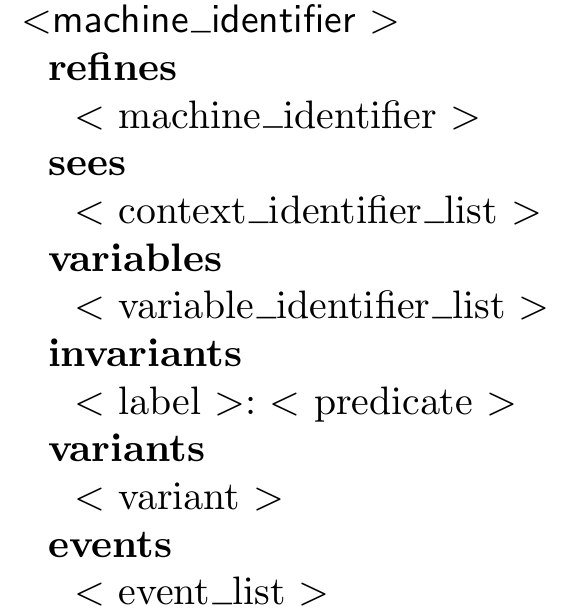
\includegraphics[width=0.4\linewidth]{event-b_machine}
  \caption{General structure of Event-B machine (taken from \cite{eventb})} 
\end{figure} 

\begin{figure}[h]
  \centering
  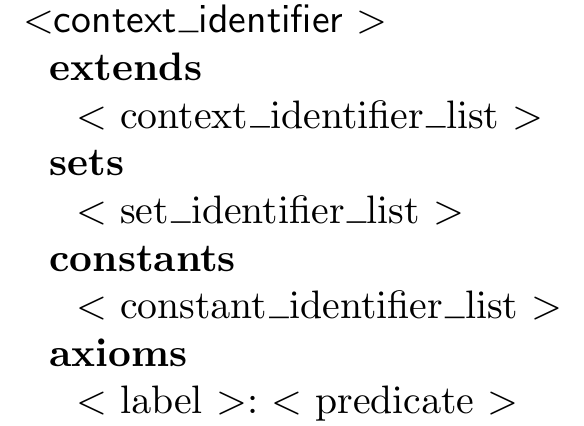
\includegraphics[width=0.4\linewidth]{event-b_context}
  \caption{General structure of Event-B context} 
\end{figure} 


\subsection{Rodin Platform}

The
\href{http://wiki.event-b.org/index.php/Main_Page}{Rodin Platform}
is an Eclipse-based IDE for Event-B that provides effective
support for refinement and mathematical proof. The platform is open source,
contributes to the Eclipse framework and is further extendable with plugins.  

